% ****** Start of file apssamp.tex ******
%
%   This file is part of the APS files in the REVTeX 4.2 distribution.
%   Version 4.2a of REVTeX, December 2014
%
%   Copyright (c) 2014 The American Physical Society.
%
%   See the REVTeX 4 README file for restrictions and more information.
%
% TeX'ing this file requires that you have AMS-LaTeX 2.0 installed
% as well as the rest of the prerequisites for REVTeX 4.2
%
% See the REVTeX 4 README file
% It also requires running BibTeX. The commands are as follows:
%
%  1)  latex apssamp.tex
%  2)  bibtex apssamp
%  3)  latex apssamp.tex
%  4)  latex apssamp.tex
%
\documentclass[%
reprint,
%superscriptaddress,
%groupedaddress,
%unsortedaddress,
%runinaddress,
%frontmatterverbose, 
%preprint,
%preprintnumbers,
%nofootinbib,
%nobibnotes,
%bibnotes,
 amsmath,amssymb,
 aps,
%pra,
%prb,
%rmp,
%prstab,
%prstper,
%floatfix,
]{revtex4-2}

\usepackage{graphicx}% Include figure files
\usepackage{dcolumn}% Align table columns on decimal point
\usepackage{bm}% bold math
\usepackage{float}
\usepackage{mathtools}
\usepackage{xcolor}
%\usepackage{hyperref}% add hypertext capabilities
%\usepackage[mathlines]{lineno}% Enable numbering of text and display math
%\linenumbers\relax % Commence numbering lines

%\usepackage[showframe,%Uncomment any one of the following lines to test 
%%scale=0.7, marginratio={1:1, 2:3}, ignoreall,% default settings
%%text={7in,10in},centering,
%%margin=1.5in,
%%total={6.5in,8.75in}, top=1.2in, left=0.9in, includefoot,
%%height=10in,a5paper,hmargin={3cm,0.8in},
%]{geometry}

\newcommand{\Hp}{\mathcal{H}}
\renewcommand{\thesection}{\arabic{section}}
\renewcommand{\thesubsection}{\arabic{subsection}}
\renewcommand{\thesubsubsection}{\arabic{subsubsection}}


\begin{document}

\section{Milestone I}

In this section we consider the evolution of the uniform background of the universe where the main goal is to use cosmological parameters to obtain observables and compare observational data. The relevant cosmological constants used in this milestone comes from 2018 Planck \cite{Planck:2018vyg} and are:
\begin{alignat*}{2}
	H_0 &= 67\,\frac{\text{km/s}}{\text{Mpc}},\hspace{5mm}N_\text{eff}&&=3.046,\\
	\Omega_{\text B0}&=0.05,\hspace{7.3mm}\Omega_{\text{CDM}0}&&=0.267,\\
	\Omega_{\text K0}&=0.00,\hspace{8mm}T_{\text{CMB}0}&&=2.7255.
\end{alignat*}
A description for each of these is given in the theory section.

\subsection{Theory}
We approximate the universe to be completely isotropic and homogeneous over large scales. This has been shown to be a reasonable assumption from observations of the CMB power spectra \cite{dodelson:2003ft}. With this we arrive at an exact solution for the metric via the Einstein field equations (EFE):
\begin{equation}
	G_{\mu\nu}+\Lambda g_{\mu\nu}=8\pi G T_{\mu\nu},\label{EFE}
\end{equation}
called the Friedmann-Robertson-Walker (FRW) metric. In flat space and Cartesian coordinates it is given by:
\[g_{\mu\nu}=\text{diag}[-c^2,a^2(t),a^2(t),a^2(t)],\]
where we are using the metric signature $(-,+,+,+)$ and $a(t)$ is the scale factor defined to be $1$ today. Since the universes expansion is strictly positive, this scale factor is an injective function w.r.t. time and can thus be used as a time measurement. In this paper we will, for computational purposes, be using the variable $x\equiv\ln(a)\implies a=e^x$. 

With the FRW metric and the EFE for a perfect liquid we derive the Friedmann equations:
\begin{align}
	\label{F1}
	\left(\frac{\dot{a}}{a}\right)^2&\equiv H^2=\frac{8\pi G}{3}\rho,\\
	\label{F2}
	\frac{\ddot{a}}{a}&=-\frac{4\pi G}{3}(\rho+3p),
\end{align}
where $\rho$ and $p$ come from the energy-momentum tensor $T_{\mu\nu}$ for a perfect liquid and is the energy density and pressure respectively of said perfect liquid. (\ref{F1}) is used to get the time dependence of the Hubble factor $H\equiv\dot{a}/a$ and is given by:
\begin{align}
	H=H_0\sqrt{\Omega_{\text M0}a^{-3}+\Omega_{\text{R}0}a^{-4}+\Omega_{\text K0}a^{-2}+\Omega_{\Lambda0}}, \label{Hubble}\\
	\Omega_{\text M0}\equiv \Omega_{B0}+\Omega_{\text{CDM}0},~~\Omega_{\text{R}0}\equiv \Omega_{\gamma0}+\Omega_{\nu0},\nonumber
\end{align}
where $\Omega_i\equiv\rho_i/\rho_C$ where $\rho_i$ is the energy density corresponding to the $i$-th particle type and $\sum_i\rho_i=\rho_C$ is the critical energy density required to have a flat universe. $\Omega_{B0},\Omega_{\text{CDM}0},\Omega_{\gamma0},\Omega_{\nu0}$ and $\Omega_{\Lambda0}$ are then the present day relative densities of baryonic matter (electrons \& protons), cold dark matter, radiation, neutrinos and dark energy respectively. The term $\Omega_{\text K0}=-kc^2/H_0$ denotes the curvature of the universe and encapsulates how said curvature affects expansion rates and energy densities. With the requirement for a flat universe we have that $\sum_i\Omega_i=1$. Since $\Omega_{\text B},\Omega_{\text{CDM}}$ and $\Omega_\gamma,\Omega_\nu$ give the same contribution to the time evolution of the Hubble parameter, we will often bundle these together as ``matter'' and ``radiation'' (or ``relativistic'') particles respectively as was done in (\ref{Hubble}).

The other Friedmann equation (\ref{F2}) is then used to describe how each component evolves with time. By approximating that particles behave like fluids we define the equation of state $\omega\equiv p/\rho$ where we have that $\omega_{\text B}=0,\omega_{\text{R}}=1/3$ and $\omega_\Lambda=-1$ for baryons, relativistic particles (photons and neutrinos) and dark energy (DE) respectively. Note that this includes the assumption that we can treat DE to be the result of a cosmological constant $\Lambda$ in the EFE. With this assumption we arrive to the following relations:
\begin{alignat}{2}
	\Omega_{\text B}(a)&=\frac{\Omega_{\text B0}}{a\Hp^2/H_0^2},\hspace{3.5mm}\Omega_{\text{CDM}}(a)&&=\frac{\Omega_{\text{CDM}0}}{a\Hp^2/H_0^2},\nonumber\\
	\Omega_{\gamma}(a)&=\frac{\Omega_{\gamma0}}{a^2\Hp^2/H_0^2},\hspace{7mm}\Omega_{\nu}(a)&&=\frac{\Omega_{\nu0}}{a^2\Hp^2/H_0^2},\label{eq:Omegai}\\
	\Omega_{\text K}(a)&=\frac{\Omega_{\text K0}}{\Hp^2/H_0^2},\hspace{10mm}\Omega_{\Lambda}(a)&&=\frac{\Omega_{\Lambda0}}{H^2/H_0^2},\nonumber
\end{alignat}
where $\Hp\equiv aH$ is the \textbf{conformal Hubble factor}. 
Two of the six density parameters follows from the observed temperature of the CMB and are given by:
\begin{align}
	\label{ORad}
	\Omega_{\gamma0}&=\frac{8\pi^3 G}{45 H_0^2}\frac{(k_BT_{\text{CMB}0})^4}{\hbar^3 c^5},\\
	\label{ONu}
	\Omega_{\nu0}&=\Omega_{\gamma0}N_{\text{eff}}\cdot\frac{7}{8}\left(\frac{4}{11}\right)^{4/3},
\end{align}
where $T_{\text{CMB}0}$ is the temperature of CMB photons today and $N_{\text{eff}}=3.046$ is the effective number of massless neutrinos. 

Further we consider the \textbf{horizon}, i.e. the ``distance'' massless particles may have travelled since the big bang. Since the universe expands this will be larger than $ct$. Considering a time $t_1$, light would have travelled a distance $d_1>ct_1$. We can then consider what $t_1$ must be such that this becomes an equality. For this we define the \textbf{conformal time} $\eta$ which, by considering the FRW line element for light-like particles, we have:
\[ds^2=0=-c^2dt^2+a^2(t)dr^2\implies \frac{dr}{dt}=\frac{c}{a},\]
from which we can define $\eta(t)\equiv\int_0^t\frac{c}{a}dt'$ and we get the differential equation:
\begin{equation}
	\frac{d\eta}{dx}=\frac{c}{\Hp},\label{detaODE}
\end{equation}
along with the initial condition $\eta(-\infty)=0$ which can be solved analytically in the radiation dominated era. Note that this condition simply states that the universe began as a singularity. We will then use the analytical solution to approximate that at some very early time, $x_\text{start}$ such that we have the new initial condition $\eta(x_\text{start})=c/\Hp(x_\text{start})$ where we will solve onwards numerically. 

Considering the same case again but allowing for spatial curvature we arrive at:
\[
r=
\begin{cases}
	\,\chi\frac{\sin(\sqrt{\left|\Omega_{\text K0}\right|}H_0\chi/c)}{\sqrt{\left|\Omega_{\text K0}\right|}H_0\chi/c},& \Omega_{\text K0}<0~\text{``Closed''}\\
	\,\chi, & \Omega_{\text K0}=0~\text{``Flat''}\\
	\,\chi\frac{\sinh(\sqrt{\left|\Omega_{\text K0}\right|}H_0\chi/c)}{\sqrt{\left|\Omega_{\text K0}\right|}H_0\chi/c},& \Omega_{\text K0}>0~\text{``Open''}
\end{cases},
\]
where we have defined the \textbf{comoving distance} $\chi\equiv\eta_0-\eta$. 

We then consider the diameter distance $d_A=D/\theta$ where $D$ is the objects physical size and $\theta$ its angular size as viewed from Earth. This can be expressed in terms of our cosmological parameters as $d_A=ar$ and from this we also acquire the  luminosity distance $d_L=r/a=d_A/a^2$. At last we consider the \textbf{cosmic time} $t$ in our $x$ coordinate:
\[t(x)=\int_0^a\frac{da}{aH}=\int_{-\infty}^0\frac{dx}{H(x)}.\]
From this we get to the ODE:
\begin{equation}
	\frac{dt}{dx}=\frac{1}{H}, \label{dtdx}
\end{equation}
with the initial condition $t(-\infty)=0$. This initial condition states that cosmic time begins once the big bang happened. As before we make an analytical approximation which gives us the initial condition $t(x_\text{start})=\frac{1}{2H(x_\text{start})}$ which is solved numerically from here.

\subsection{Implementation details}

To implement some numerical tools to solve for the background we first implement the data from (Planck) and computed the derived quantities $\Omega_{\gamma0}$ and $\Omega_{\nu0}$ with (\ref{ORad},\ref{ONu}), and $\Omega_{\Lambda0}=1-\Omega_\text{rest0}$ where ``rest'' refers to all the other $\Omega_i$.  

Next we implemented an ordinary differential equation (ODE) solver to solve the ODEs for $\eta(x)$ and $t(x)$. This was done by first setting up the respective differential equation (\ref{detaODE},\ref{dtdx}) with its corresponding initial condition, then an ODE solver was used to get a result which was then splined. The ODE solver and splining programs was already provided in the template. 

At last we computed $H(x)$ from (\ref{Hubble}) which used together with the various relations from the theory section to compute $\Hp,\frac{d\Hp}{dx},\frac{d^2\Hp}{dx^2},\Omega_i,r,d_A,d_L,\chi$ and $T_{\text{CMB}}$ all as a function of our time variable $x$. Note that the expressions for $\frac{d\Hp}{dx}$ and $\frac{d^2\Hp}{dx^2}$ were found analytically. The data was then output to a text file which was imported to Python where various plots were made.

In Python the $x$-values corresponding to radiation-matter and matter-DE equality were found by finding running a script over the data to find where the absolute value of the difference $|\Omega_i-\Omega_j|=0$. In reality they were never quite 0 due to running over a discrete index, thus we simply set some low threshold, e.g. $5\cdot10^{-5}$. To find when the universe accelerates we note that:
\[\Hp=\frac{\dot a}{a}a=\dot a\implies \frac{d\Hp}{dx}=\frac{d\Hp}{dt}\frac{dt}{dx}=\ddot{a}\frac{dt}{dx},\]
and from (\ref{dtdx}) we then have:
\[\frac{d\Hp}{dx}\equiv\Hp'=\frac{\ddot a}{H}.\]
Since $H$ is strictly positive we can then look at when $\Hp'$ changes from negative to positive. So again a Python script which runs over the indices of $\Hp$ were used to find which $x$-values this sign change happened, which corresponds to where the universe began to accelerate. 

\color{red}[2. Should we talk more about the specifics of the ODE, spiner and MCMC fit or is it simply ok to say that this is what we used and leave it as sort of a ``black box''?]\color{black}

\subsection{Tests of data}

Before considering the results it is reasonable to conduct some sanity checks on the data. We first consider $\Omega_i$ as given in FIG. \ref{Omegai}.
\begin{figure}[H]
	\caption{Time evolution of the density parameters $\Omega_i$ as a function of the scale factor $a$.}
	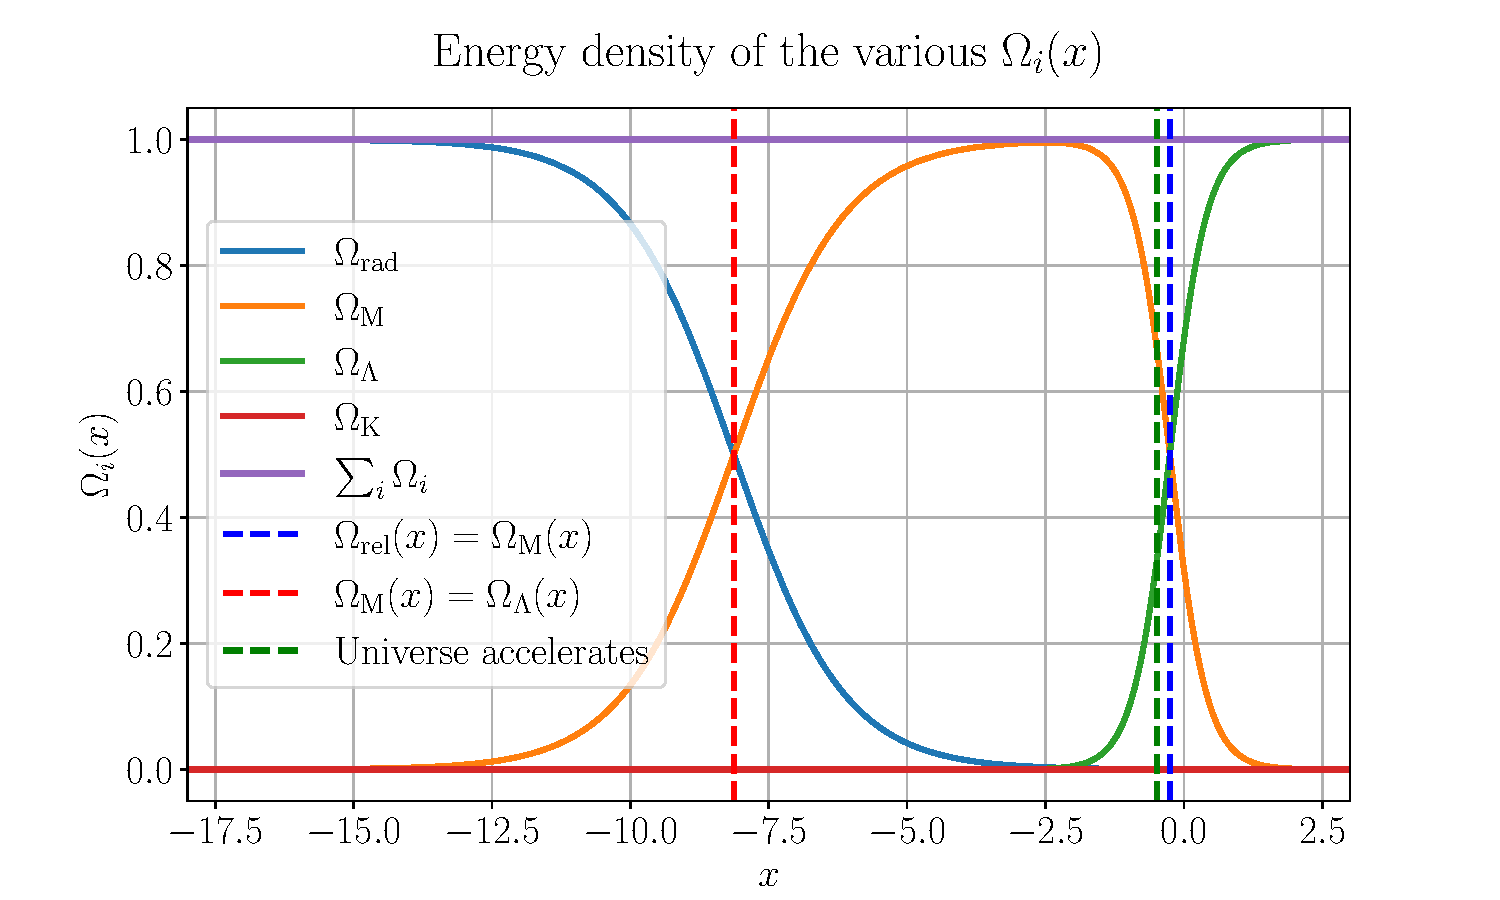
\includegraphics[width = \linewidth]{Figures/Omega_i.pdf}
	\label{Omegai}
\end{figure}
Here we can clearly see the different regimes of the various quantities. To check that the data is consistent with the analytical expressions we consider the following quantities analytically in the different regimes:
\[\frac{\Hp'}{\Hp},\hspace{5mm}\frac{1}{\Hp}\frac{d^2\Hp}{dx^2}\equiv\frac{\Hp''}{\Hp},\hspace{5mm}\frac{1}{c}\eta\Hp.\]
In the radiation dominated era where we approximate $\Omega_{\text{R}}\approx1\implies\Omega_\text{rest}\approx0$. Then by using (\ref{Hubble}) we find:
\begin{alignat*}{2}
	H_{\text{R}}(x)&\approx H_0,~~\Hp_{\text{R}}(x)&&\approx H_0e^{-x},\\
	\frac{\Hp_{\text{R}}'}{\Hp_{\text{R}}}&\approx-1,\hspace{6.5mm}\frac{\Hp_{\text{R}}''}{\Hp_{\text{R}}}&&\approx1,
\end{alignat*}
and similarly using the approximations $\Omega_{\text M}\approx1$ and $\Omega_\Lambda\approx1$ respectively, we get:
\begin{alignat*}{2}
	H_\text{M}(x)&\approx H_0e^{x/2},\hspace{5mm}\Hp_\text M(x)&&\approx H_0e^{-x/2},\\
	\frac{\Hp_\text M'}{\Hp_\text M}&\approx-1/2,\hspace{12mm}\frac{\Hp_\text M''}{\Hp_\text M}&&\approx1/4,\\
	H_\Lambda(x)&\approx H_0,\hspace{12.5mm}\Hp_\Lambda(x)&&\approx H_0e^{x},
\end{alignat*}
\vspace{-7.2mm}
\[\frac{\Hp_\Lambda'}{\Hp_\Lambda}\approx\frac{\Hp_\Lambda''}{\Hp_\Lambda}\approx1.\]
Plotting these assumptions with the data we have FIG. \ref{dHpddHp_vs_anal}. We see that there is a reasonable agreement with the analytical approximations in the given regimes. As can be seen from FIG. \ref{Omegai}, $\Omega_{\text M}\approx1$ is a relatively poor approximation compared to the others, hence larger deviations is to be expected.
\begin{figure}[h!]
	\caption{$\Hp'/\Hp$ and $\Hp''/\Hp$ compared to analytical approximations.}
	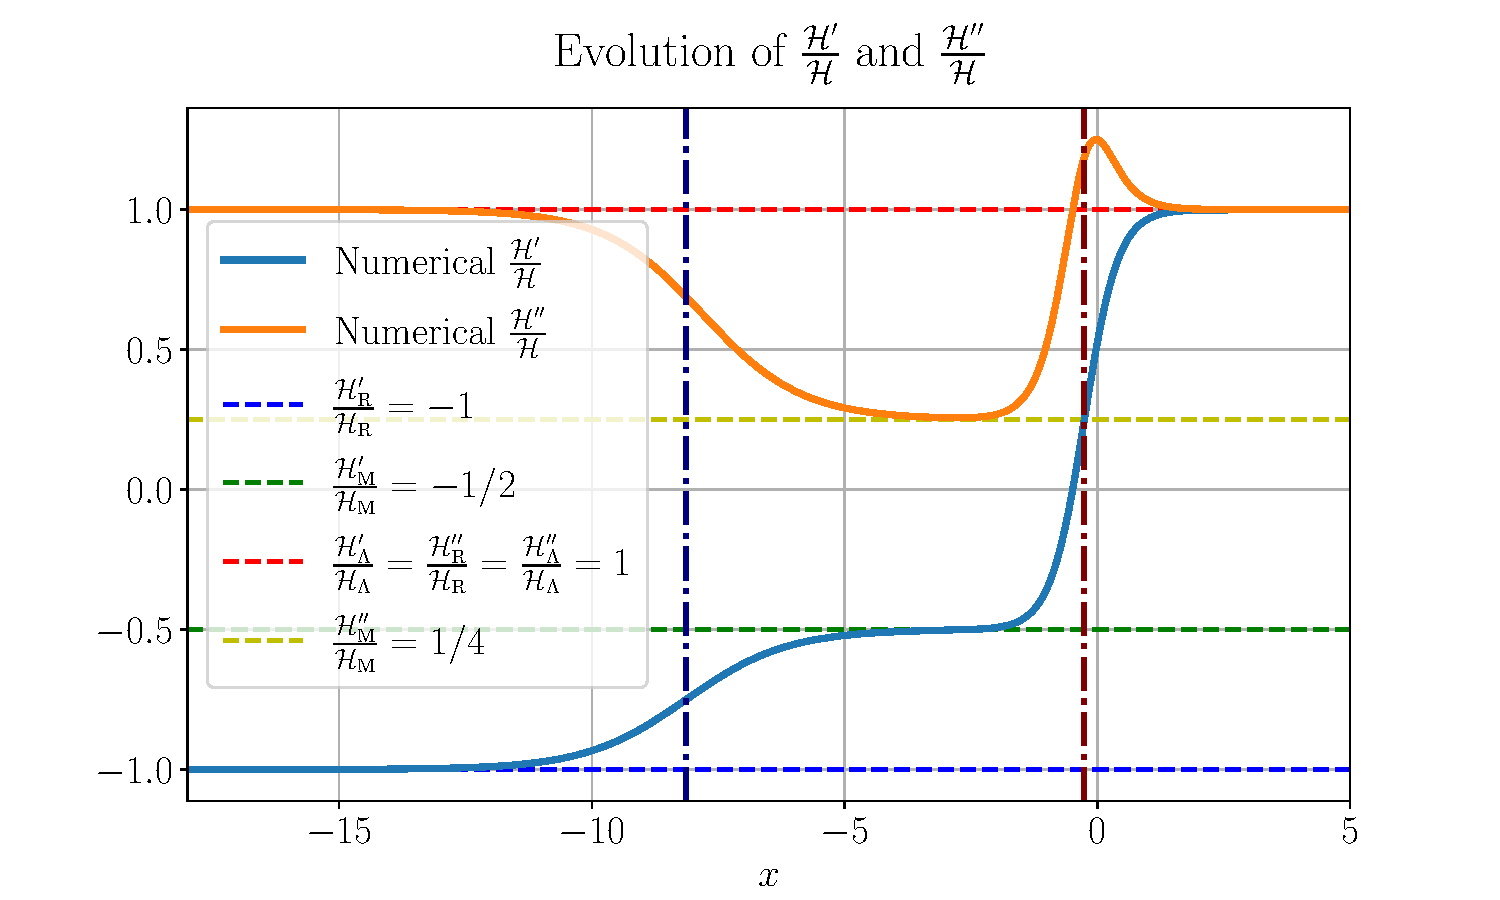
\includegraphics[width = \linewidth]{Figures/dHpddHp_vs_anal.pdf}
	\label{dHpddHp_vs_anal}
\end{figure}

Analytical approximations for the conformal time requires a little more effort. For the radiation dominated era we can solve (\ref{detaODE}) analytically:
\[\eta_\text{R}(x)=\int_{-\infty}^x\frac{c}{\Hp_\text{R}}dx'\approx\int_{-\infty}^x\frac{c}{H_0}e^{x'}dx'=\frac{c}{H_0}e^x.\]
Now we approximate this radiation dominated epoch to end abruptly at some time $x_1$ such that we can write the conformal time in the matter dominated epoch as:
\begin{align*}
	\eta_\text M(x)&\approx\eta_\text{R}(x_1)+\int_{x_1}^x\frac{c}{\Hp_\text M}dx'\\
	&\approx\frac{c}{H_0}\left(e^{x_1}+\int_{x_1}^xe^{x'/2}dx' \right)\\
	&=\frac{c}{H_0}(e^{x_1}-2e^{x_1/2}+2e^{x/2}).
\end{align*}
Again we assume that the matter dominated epoch ends abruptly at some time $x_2$ such that we can approximate:
\begin{align*}
	\eta_\Lambda(x)&\approx\eta_\text M(x_2)+\int_{x_2}^\infty\frac{c}{\Hp_\Lambda}dx'\\
	&\approx\frac{c}{H_0}\left(e^{x_1}-2e^{x_1/2}+2e^{x_1/2}+\int_{x_2}^x e^{-x'}dx' \right)\\
	&=\frac{c}{H_0}\left(e^{x_1}-2e^{x_1/2}+2e^{x_2/2}+e^{-x_2}-e^{-x} \right).
\end{align*}
Thus we find that for the various regimes we have:
\begin{align*}
	\eta_\text{R}\Hp_\text{R}/c&\approx1\\
	\eta_\text M\Hp_\text M/c&\approx(e^{x_1}-2e^{x_2/2}+2e^{x/2})e^{-x/2}\\
	\eta_\Lambda\Hp_\Lambda/c&\approx(e^{x_1}-2e^{x_1/2}+2e^{x_2/2}+e^{-x_2}-e^{-x})e^{x}.
\end{align*}
Using the $x$ values corresponding to $\Omega_{\text{R}}=\Omega_\text M$ and $\Omega_{\text M}=\Omega_\Lambda$ as the time where the respective epochs start and end we get the upper graph in FIG. \ref{eta_vs_anal_merge}.
\begin{figure}
	\caption{Numerical $\eta\Hp/c$ compared to analytical approximations in the various regimes where epochs are approximated to abruptly once $|\Omega_i-\Omega_j|=0$ and $\Omega_i<0.85$ respectively.}
	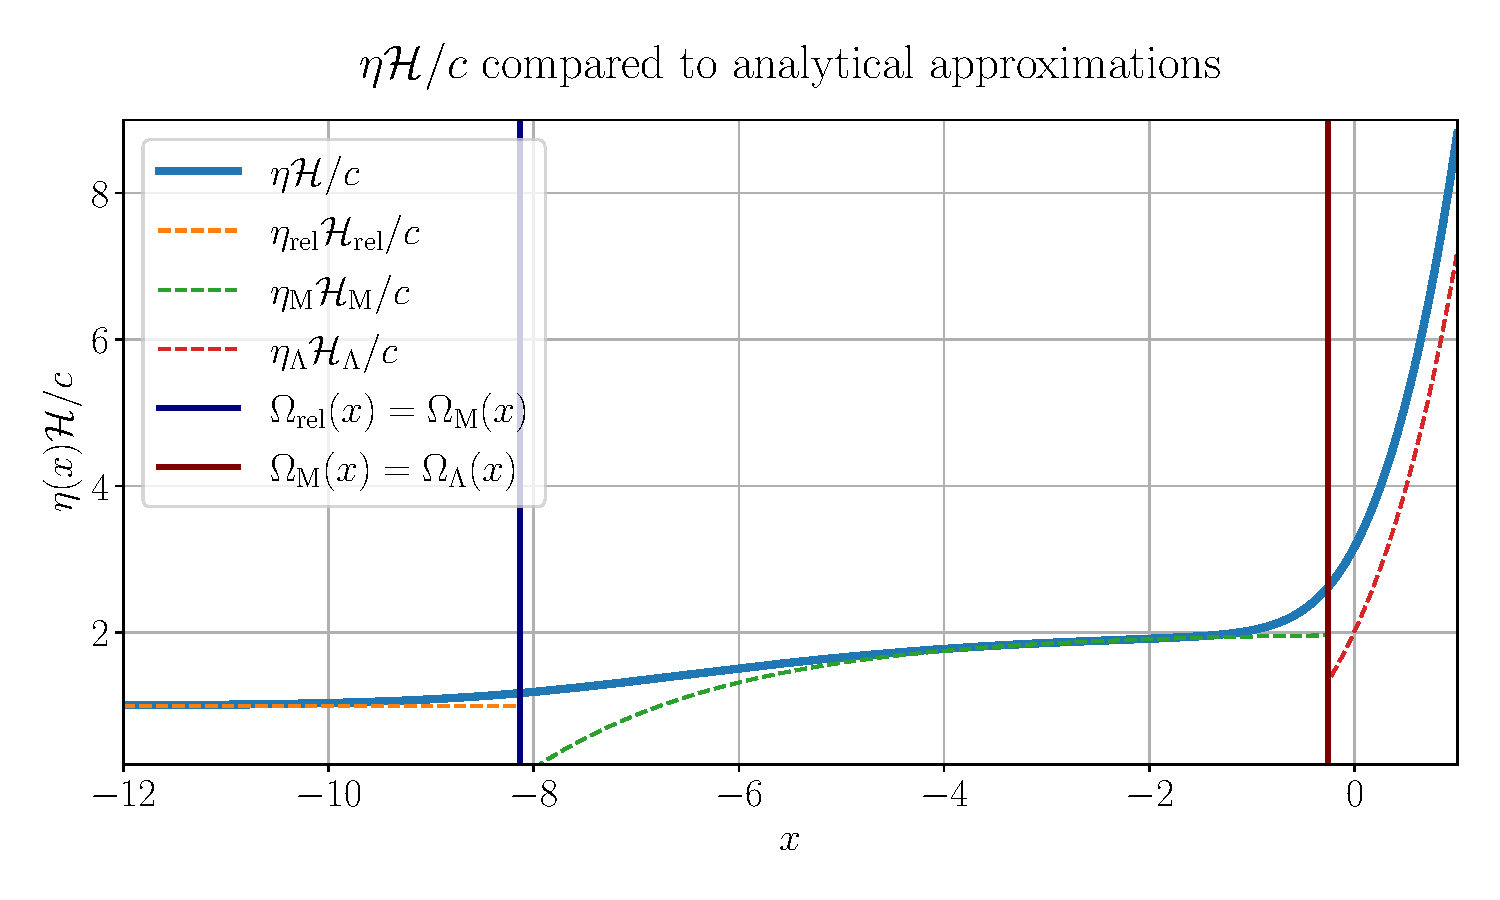
\includegraphics[width = \linewidth]{Figures/Eta_vs_anal_merge.pdf}
	\label{eta_vs_anal_merge}
\end{figure}
Clearly this approximation will be nothing close to exact due to the assumption that the epochs end abruptly when in reality the epoch's change continuously and relatively slowly. Since $\eta$ depends on how long the previous epochs lasted we can see that this heavily affects the final epoch. If we instead rather arbitrarily consider each epoch to end where the respective density parameters fall below $85\%$ then we have a plot which suits the data much better which is the lower graph in FIG. \ref{eta_vs_anal_merge}.

Overall the data seems to be consistent with the analytical expressions, even if the conformal time is a rather difficult parameter to define a solid approximation for.

\subsection{Results}

Now that the data has been stress tested to show that they are at least valid in certain regions we can go on to look at some of the results.

The time evolution of the conformal Hubble factor $\Hp(x),$ cosmic time $t(x)$ and conformal distance $\eta(x)/c$ is given in FIG. \ref{TimeEvHp}. The notable acceleration at later times in the $\Hp$ plot is due to the dark energy density exceeding $1/3$. A rough explanation for this is given later. One can also see that this same phenomena affects both the cosmic time and conformal distance inversely at the same time. This is due to them both being inversely proportional to the conformal Hubble factor.
\begin{figure}
	\caption{Time evolution of the conformal Hubble factor $\Hp$, cosmic time $t$ and conformal distance $\eta/c$ as a function of $x$.}
	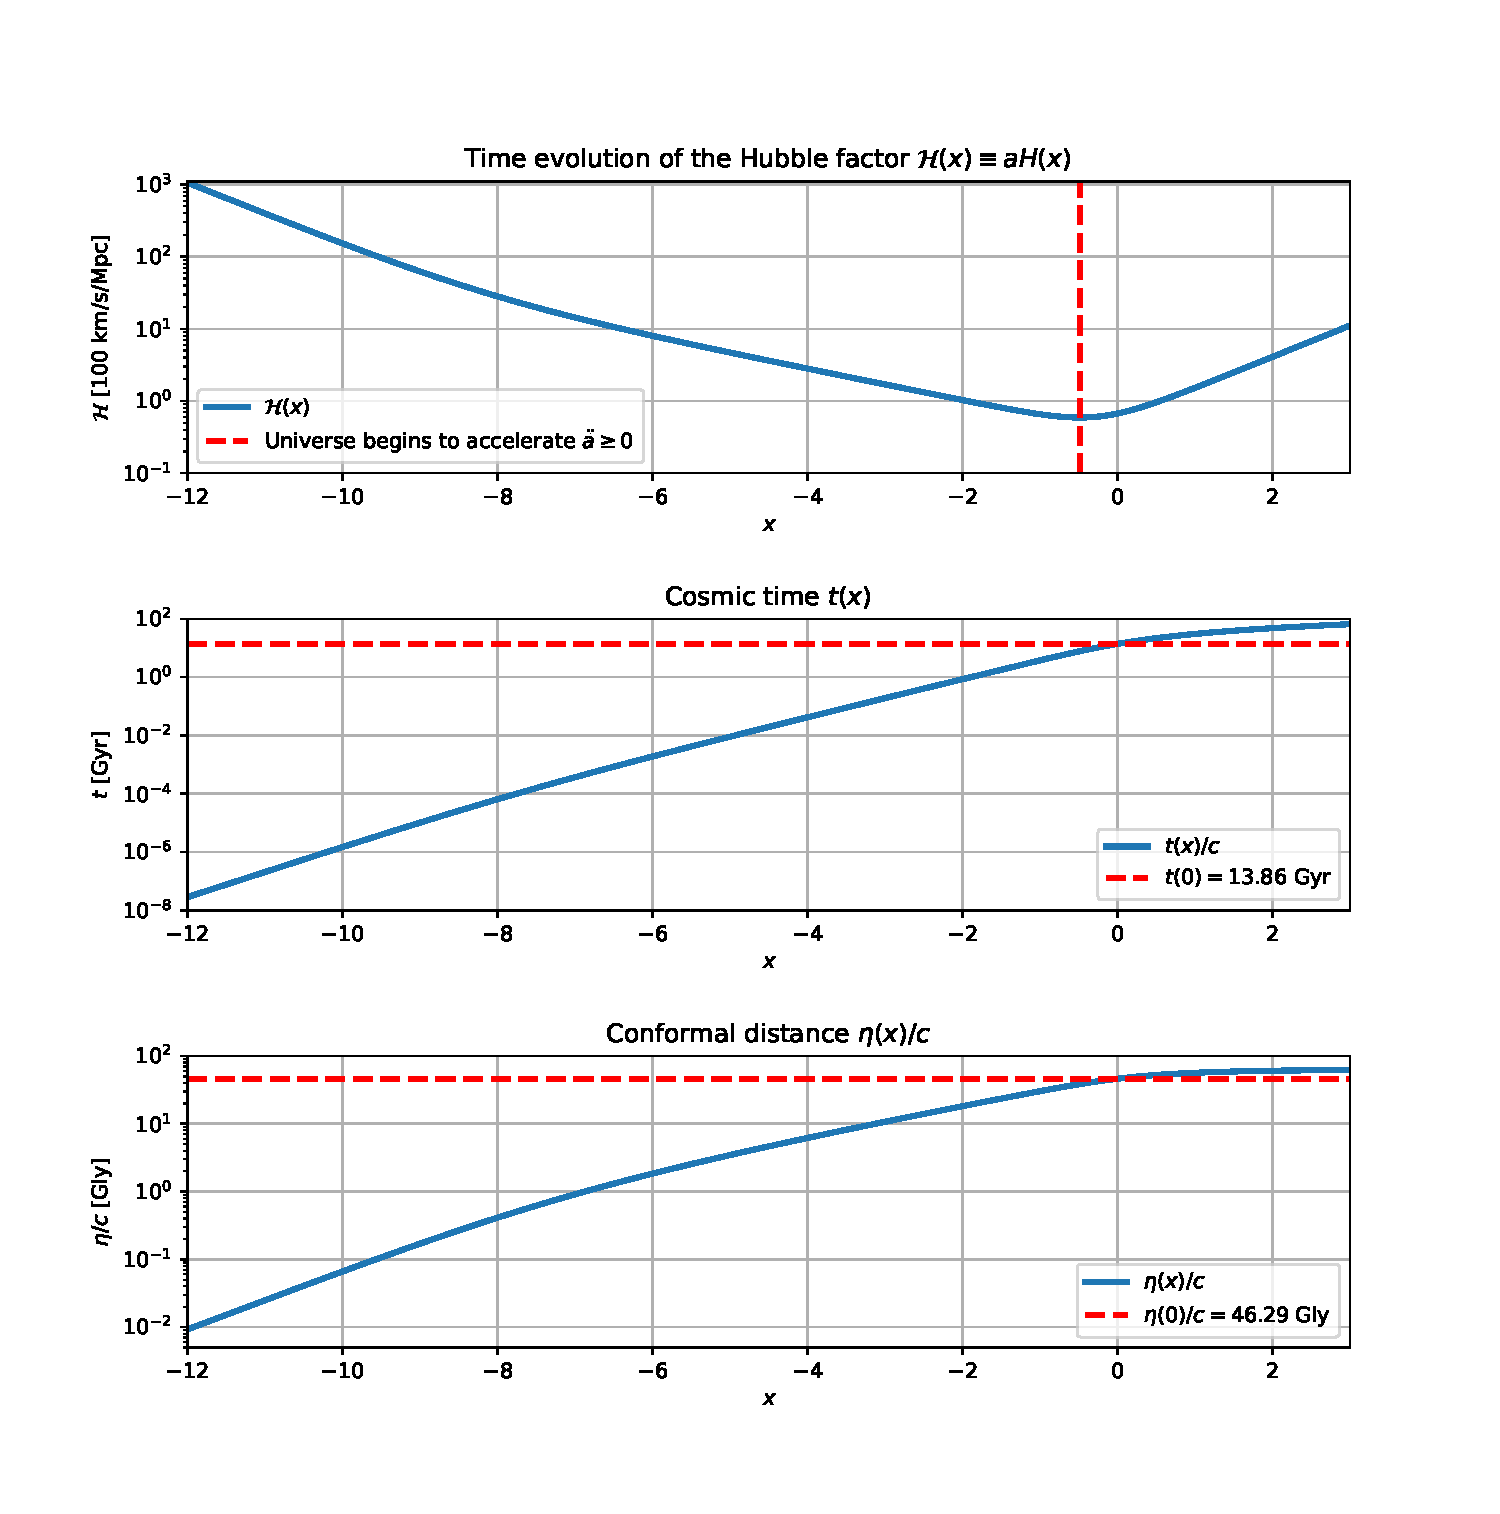
\includegraphics[width = \linewidth]{Figures/merge_Hp_t_eta_Ev.pdf}
	\label{TimeEvHp}
\end{figure}

Further we compare our data to data collected from supernova observations \cite[Betoule et al. 2014]{SDSS:2014iwm} by; comparing the luminosity distance is given in FIG. \ref{LumiDistance}, creating a Markov Chain Monte-Carlo (MCMC) fit in the $\Omega_\Lambda\Omega_\text M$-plane shown in FIG. \ref{scatt}. and making a posterior probability distribution function (PDF) of the Hubble parameter $H_0$ in FIG. \ref{PDEh}.
\begin{figure}[H]
	\caption{Luminosity distance over redshift $z$, plotted against redshift $z$ for both; our numerical data, and observational data from Betoule \cite{SDSS:2014iwm} with error-bars.}
	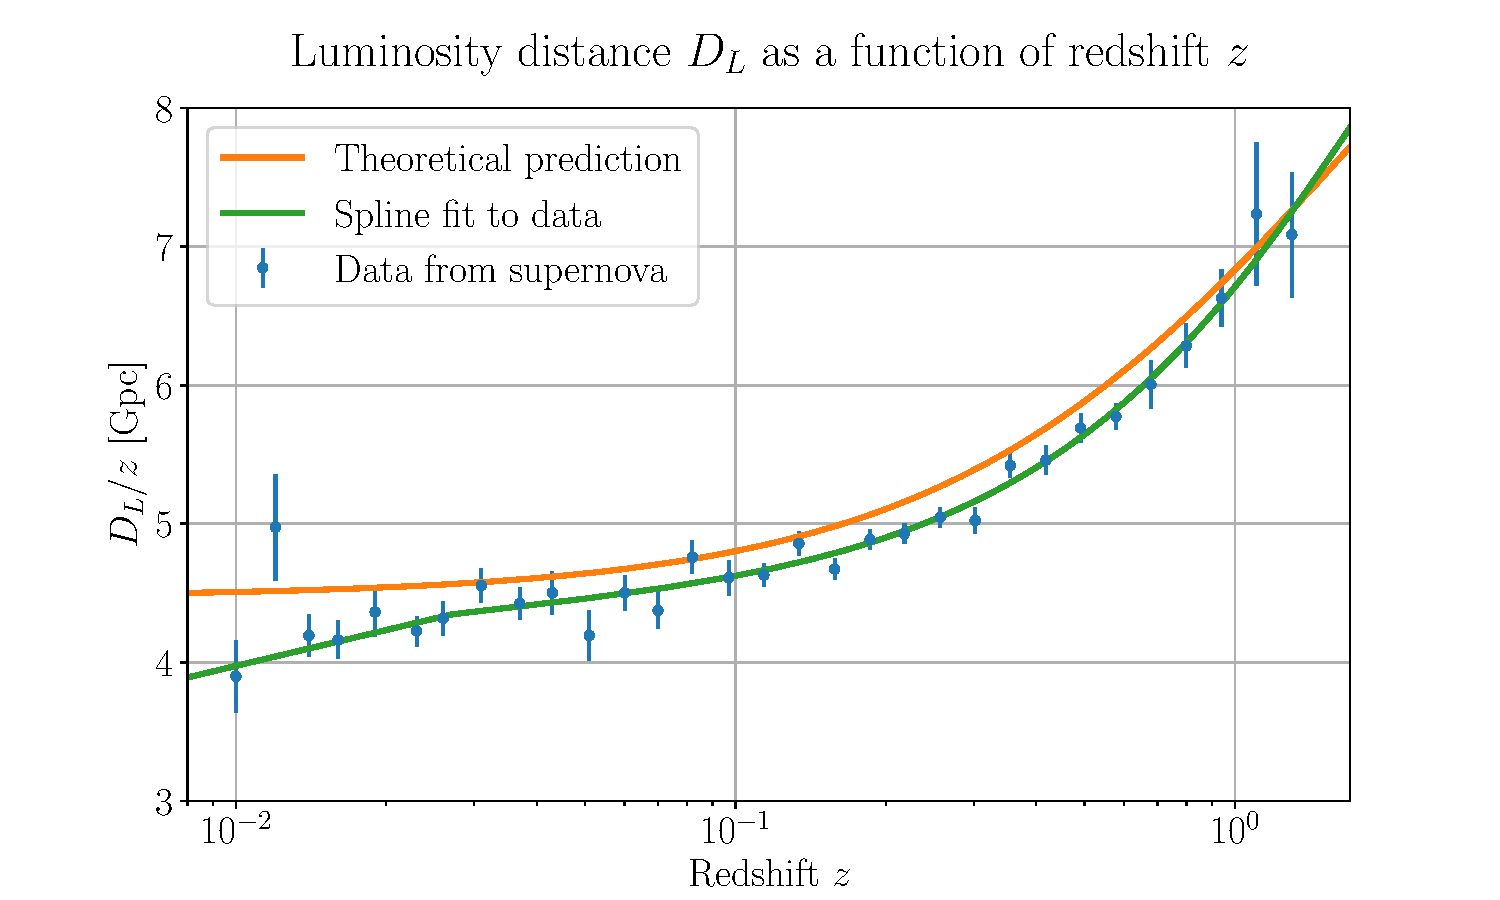
\includegraphics[width = \linewidth]{Figures/LumiDistance.pdf}
	\label{LumiDistance}
\end{figure}
\begin{figure}
	\caption{Supernova data with $1\sigma$ and $2\sigma$ constraints from MCMC fits.}
	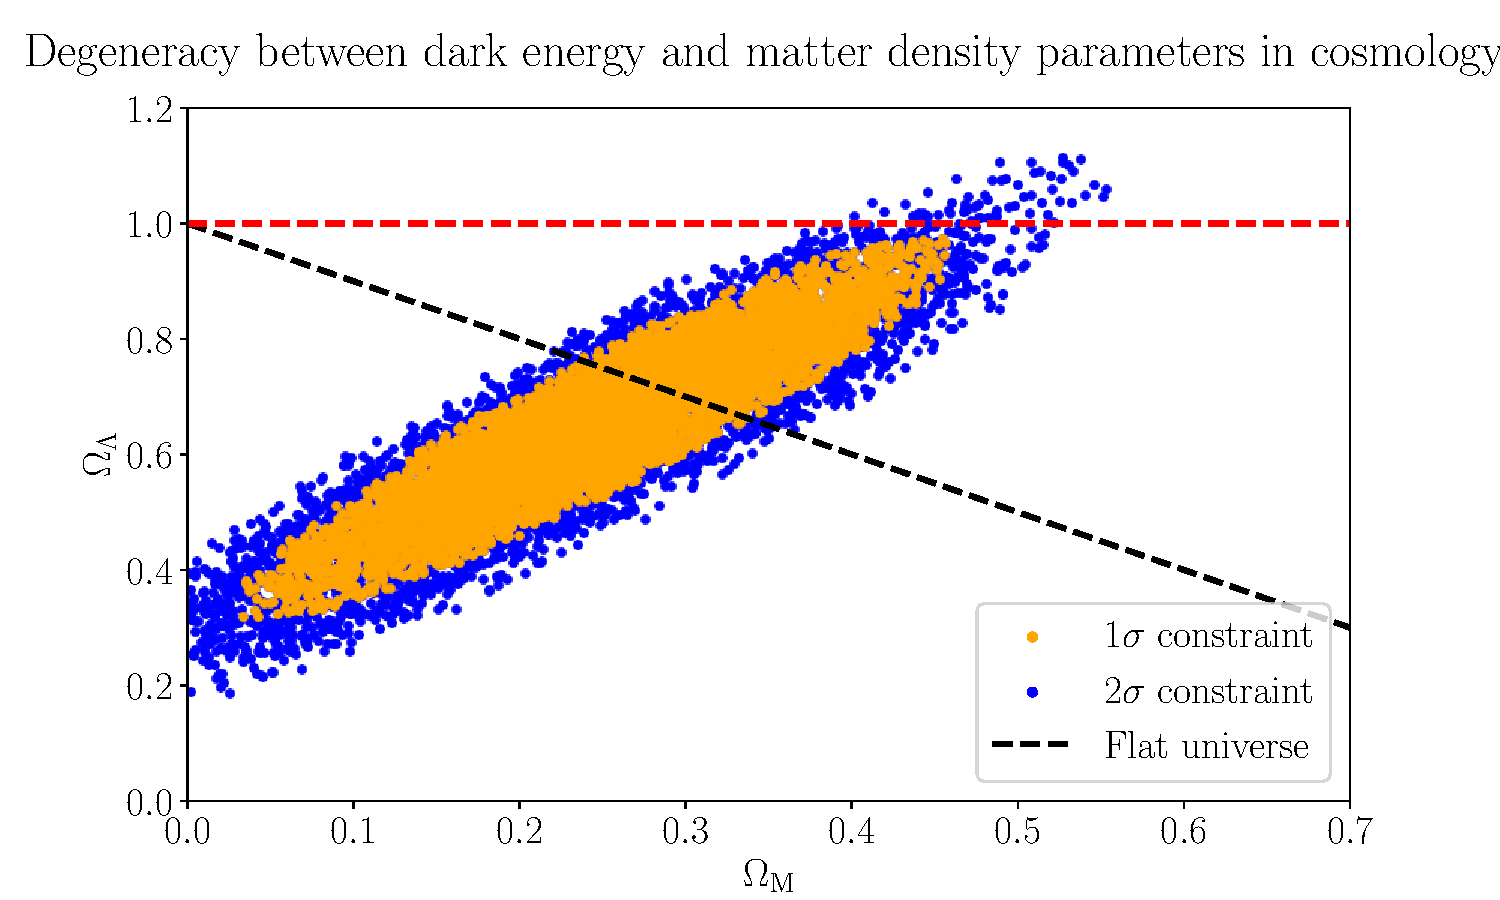
\includegraphics[width = \linewidth]{Figures/ScattPlot.pdf}
	\label{scatt}
\end{figure}
\begin{figure}
\caption{Posterior PDF of the Hubble parameter $H_0$.}
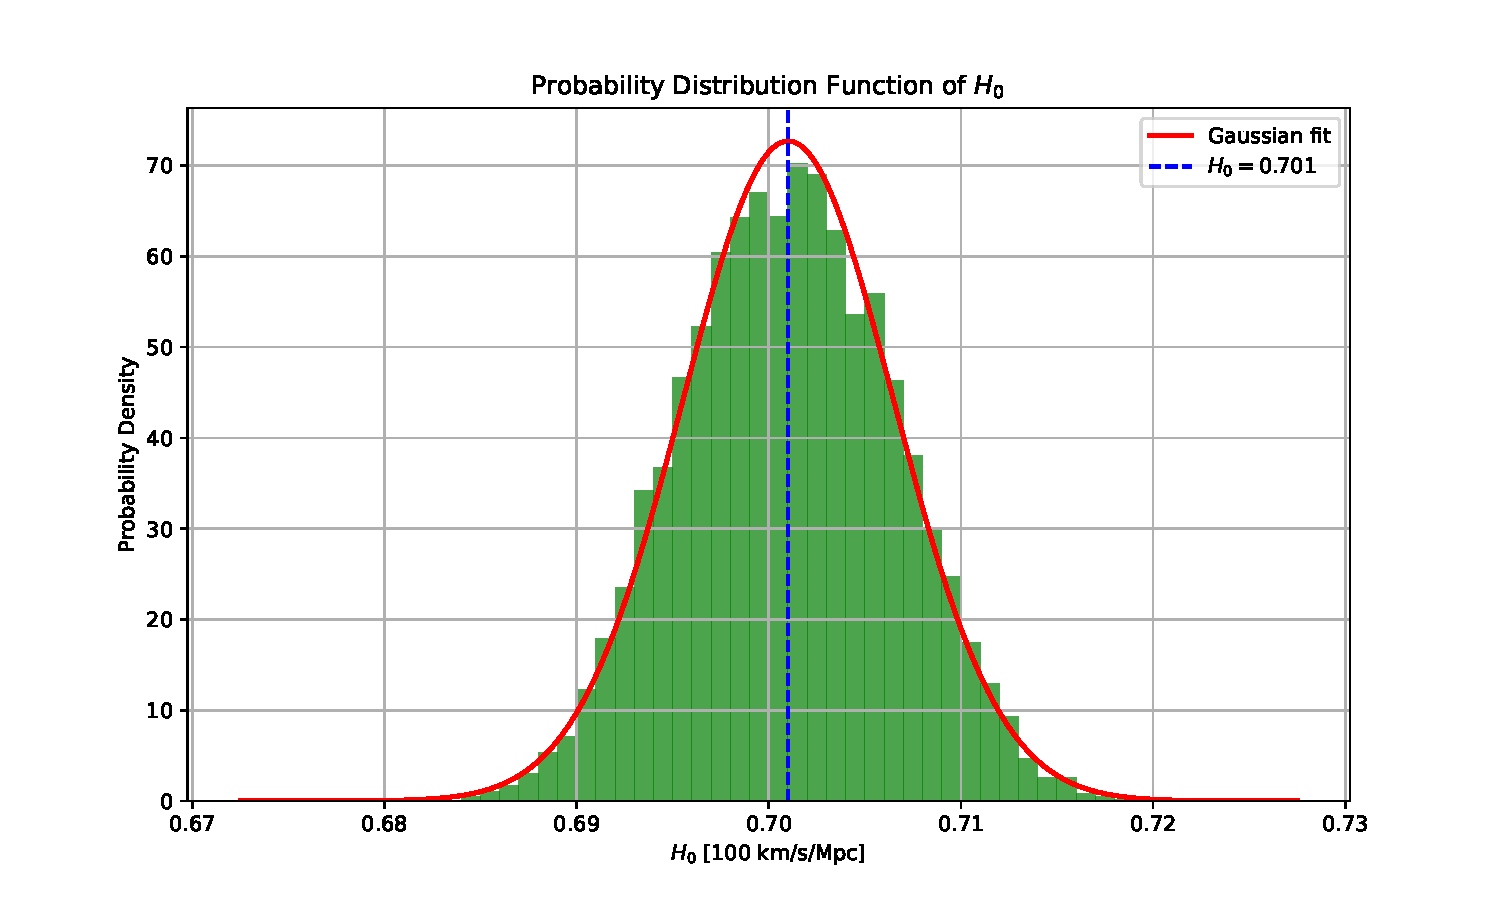
\includegraphics[width = \linewidth]{Figures/PDEh.pdf}
\label{PDEh}
\end{figure}

\color{red}[3. I tested using $h=0.701$ instead of $h=0.67$ and got a much better fit here. Is there any particular reason why we are using $h=0.67$? Is the entire point that we use something which is reasonably close and then showing that the best fit value given by the MCMC fit is better? Obviously the graph will be off if we are using an assumption for $h$ which is not accurate.]\color{black}

The luminosity distance from observational data is seemingly always lower than our data. This is likely explained by the approximations in this section not being completely valid. The scatter-plot helps us visualize the degeneracy between the density parameters, i.e. that many different combinations of $\Omega_\text M$ and $\Omega_{\Lambda}$ can yield similar observational results. This leads to rather large degenerate regions in the parameter space. In this figure we can see that the flat universe constraint significantly reduces this degeneracy by lowering the allowed parameters by multiple orders of magnitude.

Finally the posterior PDF of the Hubble parameter today $H_0$ shows that the Gaussian fit is centered at roughly $70.1\,\text{km/s/Mpc}$ which is reasonably close to other observational data (cite x) at $H_0=something$. \color{red}[4. Honestly don't know what to compare it to, there are so many different values from many different assumptions that I feel like we can just ballpark it being between 65 and 75, which doesn't seem very accurate to me.]\color{black}

Next we consider the values of $x,z,t,\eta,\Omega_\text M, \Omega_\Lambda$ and $\Omega_\text R$ at various important events. A summary of these events is given in TABLE \ref{tab:cosmo_events}.
\renewcommand{\arraystretch}{1.25}
\begin{table*} % The transpose of the table with reduced headers didn't fit double-column either :'(
	\caption{Results for cosmological parameters at various important events from numerical data. \\\color{red}[5. reasonable amount of sig figs? I used 23001 points over the interval -18 to 5 (and excluded division by 0 when needed) so that i have 3 decimals for each data point for reference.]\color{black}}
	\begin{tabular}{|l|c|c|c|c|c|c|c|}
		\hline
		Event & $x$ & $z(x)$ & $t(x)$ [Gly] & $\eta(x)/c$ [Gly] & $\Omega_\text M$ & $\Omega_{\Lambda}$ & $\Omega_{\text{Rel}}$ \\
		\hline
		Radiation-Matter Equality  & $-8.132$ & $3401$ & $5.106 \cdot 10^{-5}$ & $0.368$ & $0.500$ & $2.737 \cdot 10^{-11}$ & $0.500$ \\
		\hline
		Universe Accelerates & $-0.486$ & $0.626$ & $7.761$ & $38.55$ & $0.666$ & $0.334$ & $3.183\cdot10^{-4}$ \\
		\hline
		Matter-DE Equality & $-0.256$ & $0.292$ & $10.38$ & $42.33$ & $0.500$ & $0.500$ & $1.900\cdot10^{-4}$ \\
		\hline
		Universe Today & $0.000 $ & $0.000 $ & $13.86$ & $46.29$ & $0.317$ & $0.683$ & $9.320 \cdot 10^{-5}$ \\
		\hline
	\end{tabular}
	\label{tab:cosmo_events}
\end{table*}

The values of particular interest are $t(x=0)$ which corresponds to the age of the universe today. \cite{1} estimates this to be $13.78\pm0.20\,$Gly (Giga light years) which is reasonably close to our value of $13.86\,$Gly. 

Similarly $\eta(x=0)$ shows us the actual size of the observable universe today. Various sources (x,y,z) show that the expected conformal distance of the universe should be slightly above $46\,$Gyr, once again in agreement with the data. Another interesting point in this table is that it shows that matter and radiation equality happened about 50000 years after the big bang. Once again this is similar to other reported figures. \color{blue}[Citations missing]\color{black}

\color{blue}[This next section needs to be made more clear but is an interesting thing to note which I want to keep]\color{black}

A Final remark related to the table is to note is that the accelerating expansion of the universe happens once the dark energy density reaches $1/3$. Writing out (\ref{F1}) in terms of $\rho_i$
\[H^2=\frac{8\pi G}{3}(\rho_\text M+\rho_\text{R}+\rho_\Lambda)\]
and that in the $\Lambda$CDM model we have
\[\Omega_\Lambda=\frac{\Lambda}{3H^2}.\]
Looking back to the EFE (\ref{EFE}) then we can see that when we have $\Omega_\Lambda=\frac13$ then we can see that the cosmological constant becomes equal to the critical density of the universe. Thus this is when the universe shifts from decelerating to accelerating.

\subsection{Summary \& Conclusion}

To summarize, we numerically solved the ODEs for $\eta$ and $t$ past the radiation domination. We then computed $H(x)$ which gave us access to all the other relevant cosmological parameters. We then performed an MCMC fit with observational data from supernova events and the numerical data. Further we checked that the numerical data corresponds to analytical approximations in the different regimes. Next we introduced all the most relevant data in a graphed form in FIG \ref{TimeEvHp}-\ref{PDEh} such that important events and values were easily visualized. Finally the most relevant values were summarized in TABLE \ref{tab:cosmo_events}.

In conclusion, the data all seems to correspond quite well with observational data and previous calculations from more sophisticated methods. We then conclude that no further changes to the code is necessary to continue onto the next milestone. 


\end{document}
